\section*{Question 9}

Consider the following Markov chain on state space \( \{ 0,1, \cdots \} \).
Take \( q(k)={(1-p)}^{k-1} p, k=1,2, \cdots \) with \( 0<p<1 \).
Will this chain have a stationary distribution?
If yes, find the stationary distribution.

\begin{figure}[h]
    \centering
    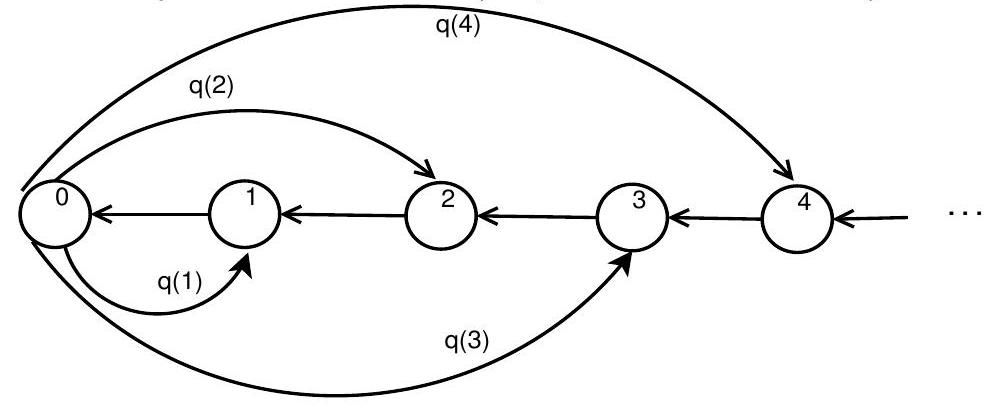
\includegraphics[width=0.8\textwidth]{figures/images/q9.jpg}
\end{figure}

\subsection*{Solution}

0 is a recurrent state.
The chain is irreducible.

Let \( \pi \) be the stationary distribution.
Then, for all \( k \geq 1 \),
\begin{align*}
    \pi(k)
     & =
    \sum_{j=0}^{\infty} \pi(j) P(j,k)
    \\
    \implies
    \pi(1)
     & =
    \pi(0) P(0,1) + \pi(1) P(1,1) + \pi(2) P(2,1) + \cdots
    \\ & =
    \pi(0) q(1) + \pi(2) q(1)
    \\ & =
    \pi(0) p + \pi(2) p
\end{align*}
